% Patricia - implementacja - zróżnicować operacje, żeby było widać co zrobiłem (wyglądają jak te same)
% Podkreślić, gdzie autorskie rozwiązania się znajdują
% Że na podstawie algorytmów dla maszyny mix wykonałem implementacje dla javy


\documentclass[aspectratio=1610,english]{beamer} %If you want to create Polish presentation, replace 'english' with 'polish' and uncomment 3-th line, i.e., '\usepackage{polski}'
\usepackage[utf8]{inputenc}
\usepackage{polski} %Uncomment for presentations in Polish
\usepackage{babel}
\usepackage{listings} %We want to put listings

%%%%%%%%%%%%%%%%%%%%%%%% Added by Jacek Oles %%%%%%%%%%%%%%%%%%%%%%%%
\usepackage{tabularx}
\graphicspath{ {./pictures/} }
\usepackage{lmodern}% http://ctan.org/pkg/lm % for proper size of $>$
\usepackage{hyperref}
\usepackage{xcolor}
\usepackage{varwidth}

\usepackage[figurename=Rysunek]{caption}
\usepackage[tablename=Tablic]{caption}
\newcommand*\rotatedBox[1]{%
	\rotatebox[origin=c]{270}{\texttt{#1}}
}
\usepackage{tikz}
\usetikzlibrary{positioning}
\usetikzlibrary{arrows.meta}
\usetikzlibrary{shapes}
\usepackage[outline]{contour}
\contourlength{2.5pt}

\def\checkmark{\tikz\fill[scale=0.4, color = AGH@green](0,.35) -- (.25,0) -- (1,.7) -- (.25,.15) -- cycle;}
%%%%%%%%%%%%%%%%%%%%%%%% Added by Jacek Oles %%%%%%%%%%%%%%%%%%%%%%%%

\mode<beamer>{ 	%in the 'beamer' mode
	\hypersetup{pdfpagemode=FullScreen}		%Enable Full screen mode
	\usetheme[nosidebar, parttitle=rightfooter]{AGH}		%Show part title in right footer
	%\usetheme[nosidebar]{AGH}				%Do not show sidebar on non-title slides
	%\usetheme[nosidebar,margins=1em]{AGH}		%Do not show sidebar on non-title slides and set both margins (left / right) to 1em
	%\usetheme[dark]{AGH}                 		%Use dark background
	%\usetheme[dark,parttitle=leftfooter]{AGH}  	%Use dark background and show part title in left footer
}
\mode<handout>{	%in the 'handout' mode
	\hypersetup{pdfpagemode=None}		
	\usepackage{pgfpages}
  	\pgfpagesuselayout{4 on 1}[a4paper,border shrink=5mm,landscape]	%show 4 slides on 1 page
  	\usetheme{boxes}
  	\addheadbox{structure}{\quad\insertpart\hfill\insertsection\hfill\insertsubsection\qquad} 	%content of header
 	\addfootbox{structure}{\quad\insertauthor\hfill\insertframenumber\hfill\insertsubtitle\qquad} 	%content of footer
}

\AtBeginPart{ %At begin part: display its name
	\frame{\partpage}
} 

\title{ 
	Projekt dyplomowy \\
	{\color{AGH@green} Implementacja drzew klasy trie} %\\
	%{\color{myDarkBlue} Implementation of trie trees}
}
\author{ Jacek Oleś\inst{1} }
\date{\tiny 28.02.2020}
\institute[Student I stopnia AGH]{
	\inst{1} 
		\tiny
		Akademia Górniczo-Hutnicza \\
		im. Stanisława Staszica w Krakowie
	\and
		\tiny
        Wydział Elektrotechniki, Automatyki, \\
        Informatyki i Inżynierii Biomedycznej
	\and
		\tiny 
		ul. Mickiewicza 30\\ 
		30-059 Kraków\\ 
		Polska 
}
\definecolor{myPurple}{RGB}{160, 27, 145}
\definecolor{myDarkBlue}{RGB}{130, 99, 232}
\definecolor{myLightBlue}{RGB}{12, 84, 178}
\lstdefinelanguage{XML}
{
  morestring=[b]",
  morestring=[s]{>}{<},
  morecomment=[s]{<?}{?>},
  stringstyle=\color{AGH@green},
  identifierstyle=\color{myPurple},
  keywordstyle=\color{myLightBlue},
  morekeywords={xmlns,version,type}% list your attributes here
}

\lstdefinestyle{myCustomStyle}{
		backgroundcolor=\color{white},   % choose the background color
        basicstyle=\fontsize{4}{5}\color{black},      % the size of the fonts that are used for the code %fontsize works only on numbers (next to rule)
		breakatwhitespace=false,         % sets if automatic breaks should only happen at whitespace
		breaklines=true,                 % sets automatic line breaking
		captionpos=b,                    % sets the caption-position to bottom
		commentstyle=\color{myPurple},      % comment style
		deletekeywords={...},            % if you want to delete keywords from the given language
		escapeinside={\%*}{*)},          % if you want to add LaTeX within your code
		extendedchars=true,              % lets you use non-ASCII characters; for 8-bits encodings only, does not work with UTF-8
		frame=single,	                   % adds a frame around the code
		keepspaces=true,                 % keeps spaces in text, useful for keeping indentation of code (possibly needs columns=flexible)
		keywordstyle=\color{blue},       % keyword style
		morekeywords={*,...},            % if you want to add more keywords to the set
		numbers=left,                    % where to put the line-numbers; possible values are (none, left, right)
		numbersep=5pt,                   % how far the line-numbers are from the code
		numberstyle=\color{lightgray},   % the style that is used for the line-numbers
		rulecolor=\color{lightgray},         % if not set, the frame-color may be changed on line-breaks within not-black text (e.g. comments (green here))
		showspaces=false,                % show spaces everywhere adding particular underscores; it overrides 'showstringspaces'
		showstringspaces=false,          % underline spaces within strings only
		showtabs=false,                  % show tabs within strings adding particular underscores
		stepnumber=1,                    % the step between two line-numbers. If it's 1, each line will be numbered
		stringstyle=\color{AGH@green},        % string literal style
		tabsize=3,	                     % sets default tabsize to 2 spaces
		title=\lstname,                  % show the filename of files included with \lstinputlisting; also try caption instead of title                                   
        language=Java,
        belowskip=-25pt,
        literate=	{ą}{{\k{a}}}1		 % needed if you want to use UTF-8 Polish chars
					{Ą}{{\k{A}}}1
					{ę}{{\k{e}}}1
					{Ę}{{\k{E}}}1
					{ó}{{\'o}}1
					{Ó}{{\'O}}1
					{ś}{{\'s}}1
					{Ś}{{\'S}}1
					{ł}{{\l{}}}1
					{Ł}{{\L{}}}1
					{ż}{{\.z}}1
					{Ż}{{\.Z}}1
					{ź}{{\'z}}1
					{Ź}{{\'Z}}1
					{ć}{{\'c}}1
					{Ć}{{\'C}}1
					{ń}{{\'n}}1
					{Ń}{{\'N}}1
}
%%%%%%%%%%% Configuration of the listings package %%%%%%%%%%%%%%%%%%%%%%%%%%
% Source: https://en.wikibooks.org/wiki/LaTeX/Source_Code_Listings#Using_the_listings_package
%%%%%%%%%%%%%%%%%%%%%%%%%%%%%%%%%%%%%%%%%%%%%%%%%%%%%%%%%%%%%%%%%%%%%%%%%%%%
\lstset{style=myCustomStyle}
%%%%%%%%%%%%%%%%%%%%%%%% Added by Jacek Oles %%%%%%%%%%%%%%%%%%%%%%%%
\newcolumntype{b}{X}
\newcommand{\centerheading}[1]{\multicolumn{1}{c}{#1}}
%	\renewcommand{\familydefault}{\rmdefault}
\renewcommand{\familydefault}{\sfdefault}

\newsavebox\runVisual
\newsavebox\runText
\newsavebox\cnfBox
\newsavebox\cnfIn
\newsavebox\cnfOut
\newsavebox\FileContent
\newsavebox\WordStrategySPTEOF
\newsavebox\WordStrategySingle
%%%%%%%%%%%%%%%%%%%%%%%% Added by Jacek Oles %%%%%%%%%%%%%%%%%%%%%%%%
%%%%%%%%%%%%%%%%%
\begin{document}
    \begin{lrbox}{\runVisual}
		\begin{varwidth}{0.8\textwidth}
			\tiny
			\begin{lstlisting}[style=myCustomStyle]
java -jar target/TrieTreeImplementations_complete_standalone.jar Visual 0 false\end{lstlisting}
		\end{varwidth}
	\end{lrbox}
	
    \begin{lrbox}{\runText}
		\begin{varwidth}{0.8\textwidth}
			\tiny
			\begin{lstlisting}[style=myCustomStyle]
java -jar target/TrieTreeImplementations_complete_standalone.jar Text 9 true\end{lstlisting}
		\end{varwidth}
	\end{lrbox}
	
    \begin{lrbox}{\cnfBox}
		\begin{varwidth}{0.2\textwidth}
		        \fontsize{6pt}{6pt}\selectfont
    			\begin{lstlisting}[mathescape=true]
/***
// [...]
***/
$v_{7272} \land$
$v_{30549} \land$
$v_{7270} \land$
$v_{30550} \land$
$v_{30551} \land$
$v_{30552} \land$
$v_{7314} \land$
$v_{30553} \land$
$v_{7268} \land$
$v_{7267} \land$
// [...]
$(\neg v_{31503} \lor \neg v_{442} \lor \neg v_{24184}) \land$
$(v_{31503} \lor \neg v_{442} \lor v_{24184}) \land$
$(v_{31503} \lor v_{442} \lor \neg v_{24184})$
// [...]
\end{lstlisting}
		\end{varwidth}
	\end{lrbox}
	
    \begin{lrbox}{\cnfIn}
		\begin{varwidth}{0.25\textwidth}
		        \fontsize{6pt}{6pt}\selectfont
    			\begin{lstlisting}[]
c 100 20
// [...]
p cnf 31503 94748
7272 0
30549 0
7270 0
30550 0
30551 0
30552 0
7314 0
30553 0
7268 0
7267 0
// [...]
-31503 -442 -24184 0
31503 -442 24184 0
31503 442 -24184 0
// NL at the end of file\end{lstlisting}
		\end{varwidth}
	\end{lrbox}

    \begin{lrbox}{\cnfOut}
		\begin{varwidth}{0.625\textwidth}
		        \fontsize{5pt}{5pt}\selectfont
    			\begin{lstlisting}[]
7272_0|30549_0|7270_0|30550_0|30551_0|30552_0|7314_0|30553_0|7268_0|7267_0|/***
        [...]
***/-31503_-24184_-442_0|-442_24184_31503_0|-24184_442_31503_0|;\end{lstlisting}
		\end{varwidth}
	\end{lrbox}
	
    \begin{lrbox}{\FileContent}
		\begin{varwidth}{\textwidth}
			\tiny
			\begin{lstlisting}[style=myCustomStyle]
"THIS IS THE HOUSE THAT JACK BUILT;"\end{lstlisting}
		\end{varwidth}
	\end{lrbox}
	
    \begin{lrbox}{\WordStrategySPTEOF}
		\begin{varwidth}{0.5\textwidth}
			\tiny
			\begin{lstlisting}[style=myCustomStyle]
"THIS IS THE HOUSE THAT JACK BUILT;"
"IS THE HOUSE THAT JACK BUILT;"
"THE HOUSE THAT JACK BUILT;"
"HOUSE THAT JACK BUILT;"
"THAT JACK BUILT;"
"JACK BUILT;"
"BUILT;"\end{lstlisting}
		\end{varwidth}
	\end{lrbox}
		
    \begin{lrbox}{\WordStrategySingle}
		\begin{varwidth}{0.5\textwidth}
			\tiny
			\begin{lstlisting}[style=myCustomStyle]
"THIS "
"IS "
"THE "
"HOUSE "
"THAT "
"JACK "
"BUILT;"\end{lstlisting}
		\end{varwidth}
	\end{lrbox}
	
  	\maketitle
  	
  	%%%%%%%%%%%%%%%%%%%%%%%%%%%
%   	\begin{frame}{Spis treści}
%   		\tableofcontents
%   	\end{frame}
    %%%%%%%%%%%%%%%%%%%%%%%%%%%
  	\section{Cele, hipoteza oraz motywacje pracy}
  	%%%%%%%%%%%%%%%%%%%%%%%%%%%
	\begin{frame}{Cele pracy i ich motywacje}{}
	    \begin{enumerate}
	        \item Cele:
                \begin{itemize}
                    \footnotesize
                    \item {\color{AGH@green}Analiza algorytmów} dotyczących {\color{AGH@green}drzewa \emph{Trie}} (tworzenie, przeszukiwanie)
                    \item {\color{AGH@green}Implementacja} algorytmów dotyczących wybranego rodzaju {\color{AGH@green}drzewa} ({\color{AGH@green}\emph{Patricia}}) w języku \emph{Java}
                \end{itemize}
	        
	        \item Motywacja celów:
	            \begin{itemize}
                    \footnotesize
	                \item {\color{AGH@green}Rozjaśnienie i uściślenie pojęć} związanych z pojęciem {\color{AGH@green}\emph{Trie}} (oraz {\color{AGH@green}\emph{Patricia}}), {\color{AGH@green}gdyż:}
	                \begin{itemize}
                        \footnotesize
    	                \item {\color{AGH@green}\emph{Trie} to często pojawiające się pojęcie} w literaturze oraz innych źródłach. 
    	                \item {\color{AGH@green}Wielokrotnie} zostaje {\color{AGH@green}przedstawione powierzchniowo}, pobieżnie. 
	                \end{itemize}
	            \end{itemize}
	    \end{enumerate}
	\end{frame}
	
	\begin{frame}{Hipoteza pracy i motywacja za nią}
	    \vspace*{-0.35cm} 
	    \begin{enumerate}
	        \addtolength{\itemindent}{-0.75cm}
	        \item Hipoteza
            \begin{itemize}
	            \addtolength{\itemindent}{-0.75cm}
                \item {\color{AGH@green} Jest możliwym modyfikacja 3 algorytmów} Knuth'a - dotyczące drzewa \emph{Patricia} - {\color{AGH@green}tak, aby:}
                \begin{itemize}
	                \addtolength{\itemindent}{-0.75cm}
                    \item {\color{AGH@green}Klucze mogły przyjmować postać pojedynczego słowa;} 
                    \item {\color{AGH@green}Pozwalając} (jednocześnie) {\color{AGH@green}użytkownikowi na wybór strategii definiującej postać klucza.}
                \end{itemize}
            \end{itemize}
	       
	       \item Motywacja hipotezy
	            \begin{itemize}
	                \addtolength{\itemindent}{-0.75cm}
	                \item {\color{AGH@green}Chęć ujednolicenia pojęcia klucza}; 
	                \item {\color{AGH@green}Gdyż przyjmował on wyróżniającą się postać} na tle pozostałych algorytmów \newline 
	                \hspace*{-0.75cm} zaproponowanych przez Knuth'a. 
	            \end{itemize} 
	    \end{enumerate}
	    
        \color{gray}
        \centering
        \usebox\FileContent \scriptsize \newline
        
        Plik źródłowy drzewa Patricia
        \vspace*{0.3cm}
	    \begin{columns}
	        \column{0.5\textwidth}
	            \centering
	            \usebox\WordStrategySPTEOF \newline
	            
	            \vspace*{0.1cm}
	            \scriptsize Postać klucza według algorytmów Knuth'a \newline
	            Strategia 1: Start Position To End Of File
	        \column{0.5\textwidth}
	            \centering
	            \usebox\WordStrategySingle \newline
	            
	            \vspace*{0.1cm}
	            \scriptsize Klucz postaci pojedynczego słowa \newline
	            Strategia 2: Single Word
	    \end{columns}
	\end{frame}
  	%%%%%%%%%%%%%%%%%%%%%%%%%%%
  	\section{Opracowanie teoretyczne}
  	%%%%%%%%%%%%%%%%%%%%%%%%%%%
	\begin{frame}{Opracowanie teoretyczne}{}
	    \begin{columns}
	        \hspace*{-0.75cm}
	        \column{0.8\textwidth}
        	    \begin{enumerate}
        	        \item Opracowanie teoretyczne zawiera przedstawienie:
        	        \begin{enumerate}
            	        \item {\color{AGH@green}historii terminu} \emph{Trie},
            	        \item {\color{AGH@green}abstraktu struktury} drzewa \emph{Trie},
            	        \item {\color{AGH@green}10 operacji} możliwych do wykonania na drzewie \emph{Trie},
            	        \item {\color{AGH@green}5 wariacji} struktury {\color{AGH@green}drzewa} \emph{Trie},
            	        \item zagadnienia {\color{AGH@green}koniunkcyjnej postaci normalnej}.
        	        \end{enumerate}
        	        
        	        \item Wykorzystując:
                    \begin{enumerate}
                        \item książkę {\color{AGH@green},,Sztuka programowania`` Donalda E. Knuth'a}; \newline
                        {   \scriptsize \color{gray}
                                \hspace*{0.9cm} Cały rozdział ,,Przeszukiwanie cyfrowe`` oraz ćwiczenia z nim powiązane;
                        }
                        \item oraz dodatkowych {\color{AGH@green}30 źródeł}.
                    \end{enumerate}
        	    \end{enumerate}
	        \column{0.2\textwidth}
                \includegraphics[width=\textwidth]{KnuthBookCover.png}
	    \end{columns}
	\end{frame}
    %%%%%%%%%%%%%%%%%%%%%%%%%%%
  	\section{Przedstawienie zagadnień}
  	%%%%%%%%%%%%%%%%%%%%%%%%%%%
	\begin{frame}{Drzewa \emph{Trie}}{Przedstawienie zagadnień}
	   {\color{AGH@green}Drzewo \emph{Trie}} - drzewo poszukiwań przechowujące w węzłach fragmenty kluczy \newline
	   % \begin{columns}
	   %     \column{0.8\textwidth}
    	        {   \small \color{gray}
        	        Drzewo stopnia $M$ {\color{gray} {\color{gray}(\emph{M-ary} lub \emph{M-way})}} \newline
                    {   \scriptsize \color{lightgray}
                        \hspace*{0.9cm} Drzewo, którego węzły posiadają co najwyżej $M$ dzieci;
                    }
    	            \begin{enumerate} 
    	                \footnotesize \color{gray}
    	                \item Każdy węzeł może być reprezentowany w postaci $M$-elementowych wektorów.
        	            \item Komórki wektorów przyporządkowane są do poszczególnych $M$ znaków, \newline 
        	            $M$ elementowego alfabetu.
        	            \item Każda z komórek {\color{lightgray}(znak jej przyporządkowany)} pozwala na przejście gałęzią z węzła na węzeł na następnym poziomie.
    	            \end{enumerate}
    	        }
	       % \column{0.3\textwidth}
	       \vspace*{-0.7cm}
        	    \begin{figure}[H]
        	       % \caption{Drzewo trie}\label{fig:DrzewoTrie}
            	    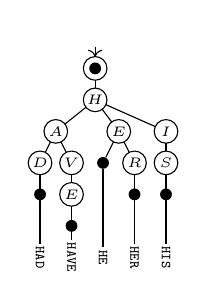
\begin{tikzpicture}[
            	    start/.style = {},
            		state/.style = { circle, top color = white, bottom color = white, draw, black, text = black, minimum width = 0.3 cm, font = \tiny, inner sep=0pt, outer sep=0pt },
            		comp/.style = {font = \tiny, inner sep=0.5pt, outer sep=0.5pt},
            		end/.style = { circle, fill, color = black, inner sep=0pt, minimum width = 0.15 cm },
            		]
            		\def\oneUnit{0.2cm}
            		
            		\node[start] (START) at (-9*\oneUnit,8*\oneUnit) {};
            		
            		\node[state] (ROOT) at (-9*\oneUnit,6*\oneUnit) {};
            		\node[end] (ROOTend) at (-9*\oneUnit,6*\oneUnit) {};
            		
            		\node[state] (H) at (-9*\oneUnit,4*\oneUnit) {$H$};
            		
		            \node[state] (A21) at (-11.5*\oneUnit,2*\oneUnit) {$A$};
            		\node[state] (E2) at (-7.5*\oneUnit,2*\oneUnit) {$E$};
            		\node[state] (I21) at (-4.5*\oneUnit,2*\oneUnit) {$I$};
            		
            		\node[state] (D3) at (-12.5*\oneUnit,0*\oneUnit) {$D$};
            		\node[state] (V3) at (-10.5*\oneUnit,0*\oneUnit) {$V$};
            		\node[end] (HeEnd) at (-8.5*\oneUnit,0*\oneUnit) {};
            		\node[state] (R3) at (-6.5*\oneUnit,0*\oneUnit) {$R$};
            		\node[state] (S31) at (-4.5*\oneUnit,0*\oneUnit) {$S$};
            		
            		\node[end] (HadEnd) at (-12.5*\oneUnit,-2*\oneUnit) {};
            		\node[state] (E4) at (-10.5*\oneUnit,-2*\oneUnit) {$E$};
            		\node[end] (HerEnd) at (-6.5*\oneUnit,-2*\oneUnit) {};
            		\node[end] (HisEnd) at (-4.5*\oneUnit,-2*\oneUnit) {};
            		
            		\node[end] (HaveEnd) at (-10.5*\oneUnit,-4*\oneUnit) {};
		
            		\node[comp] (compHAD) at (-12.5*\oneUnit,-6*\oneUnit) {\rotatedBox{HAD}};
            		\node[comp] (compHAVE) at (-10.5*\oneUnit,-6*\oneUnit) {\rotatedBox{HAVE}};
            		\node[comp] (compHE) at (-8.5*\oneUnit,-6*\oneUnit) {\rotatedBox{HE}};
            		\node[comp] (compHER) at (-6.5*\oneUnit,-6*\oneUnit) {\rotatedBox{HER}};
            		\node[comp] (compHIS) at (-4.5*\oneUnit,-6*\oneUnit) {\rotatedBox{HIS}};
            		
    				\path[->] (START) edge [] (ROOT);
            		
    				\path (ROOT) edge [] (H);
    				
    				\path (H) edge [] (A21);
            		\path (H) edge [] (E2);
            		\path (H) edge [] (I21);
            		
    				\path (A21) edge [] (D3);
            		\path (A21) edge [] (V3);
            		\path (E2) edge [] (HeEnd);
            		\path (E2) edge [] (R3);
            		\path (I21) edge [] (S31);
            		
            		\path (D3) edge [] (compHAD);
            		\path (V3) edge [] (E4);
            		\path (HeEnd) edge [] (compHE);
            		\path (R3) edge [] (compHER);
            		\path (S31) edge [] (compHIS);
            		
            		\path (E4) edge [] (compHAVE);
            		
            		\end{tikzpicture}
            		
            		\centering
            		\footnotesize
            		
\begin{tikzpicture}[
                	    start/.style = {},
                		state/.style = { circle, top color = white, bottom color = white, draw, black, text = black, minimum width = 0.3 cm, font = \tiny, inner sep=0pt, outer sep=0pt },
                		comp/.style = {font = \tiny, inner sep=0.5pt, outer sep=0.5pt},
                		end/.style = { circle, fill, color = black, inner sep=0pt, minimum width = 0.15 cm },
            		] 
            		    \node[end] (End) at (0,0) {}; 
            		    \node at (1.25,0.05) {\tiny znak końca słowa};
            		\end{tikzpicture} 
            		
            		\centering
            		\begin{tikzpicture}[
                	    start/.style = {},
                		state/.style = { circle, top color = white, bottom color = white, draw, black, text = black, minimum width = 0.3 cm, font = \tiny, inner sep=0pt, outer sep=0pt },
                		comp/.style = {font = \tiny, inner sep=0.5pt, outer sep=0.5pt},
                		end/.style = { circle, fill, color = black, inner sep=0pt, minimum width = 0.15 cm },
            		] 
            		    \node[state] (StartOuter) at (0,0) {}; 
            		    \node[end] (StartInner) at (0,0) {}; 
            		    \node at (1.3,0.005) {\tiny znak węzeł korzeń};
            		\end{tikzpicture}
        	    \end{figure}
        % \end{columns}
	\end{frame}
	%%%%%%%%%%%%%%%%%%%%%%%%%%%
	\begin{frame}{Drzewa \emph{Patricia}}{Przedstawienie zagadnień}
	    \begin{columns}
	        \column{0.6\textwidth}
	            {   \footnotesize
        	        Drzewo \emph{Patricia} to {\color{AGH@green} wariacja drzewa \emph{Trie}}.
        	        \begin{itemize}
        	            \scriptsize
        	            \item {\color{AGH@green} Przechowuje klucze w} postaci {\color{AGH@green} zawartości pliku}.
        	            \item Sama {\color{AGH@green} struktura przechowuje odniesienia do pozycji w pliku}.
        	            \item Wstępnie {\color{AGH@green} porównuje} tylko {\color{AGH@green} bity rozróżniające klucze} zawarte w drzewie.
        	            \item {\color{AGH@green} Na końcu porównuje zgodność wszystkich bitów wstępnie dopasowanego klucza} z bitami argumentu przeszukiwania.
    	            \end{itemize}%
	            }%
%%%%%%%%%%%%%%%%%%%%%%%%%%%%%%%%%%%%%%%%%%%%%%%%%%%%%%%%%%%%%%%%%%%%%%%%%%%%%%%%%%%%%%%%%%%%%%%%%%%%%%%%%%%%%%%%%%%%%%%%%%%%%%%%%%%%%%%%%%%%%%%%%%%%%%%%%%%%%%%%%%%%%%%%%%%%%%%%%%%%%%%%%%%%%%%%%%%%%%%%%%%%%%%%%%%%%%%%%%%%%%%%%%%%%%%%%%%%%%%%%%%%%%%%%%%%%%%%%%%%%%%%%%%%%%%%%%%%%%%%%%%%%%%%%%%%%%%%%%%%%%%%%%%%%%%%%%%%%%%%%%%%%
\vspace*{-0.3cm}%
% 
                \begin{figure}
        		    \centering
    		        \begin{tikzpicture}[
                	    >={Stealth[inset=0pt,length=4pt, angle'=25,round]},
                		nodeBox/.style = { rectangle, top color = white, bottom color = white, draw, black, text = black, minimum width = 0.8 cm, minimum height = 0.8 cm, font = \tiny, inner sep=0.05cm, outer sep=0.05cm },
                		word/.style = { font = \tiny, inner sep=0.5pt, outer sep=0.5pt, text = black },
                		greekSymbol/.style = { ellipse, minimum width = 0.35 cm, minimum height = 0.35 cm, fill, color = black, font = \tiny, inner sep=0pt, outer sep = 0pt, text = white },
                		position/.style = { ellipse, minimum width = 0.35 cm, minimum height = 0.35 cm, top color = white, bottom color = white, draw, black, font = \tiny, inner sep=0pt, outer sep = 0pt, text = black},
    		        ]
	\def\oneUnit{0.6cm}
	
	\node[nodeBox] (LEGENDskip) at (0*\oneUnit,0*\oneUnit) {-1};
	\node[greekSymbol] (LEGENDsymbol) at (-0.35*\oneUnit, 0.35*\oneUnit) {$L$};
	\node[position] (LEGENDposition) at (0.35*\oneUnit, 0.35*\oneUnit) {0};
	\node[word] (LEGEND) at (0*\oneUnit, -0.35*\oneUnit) {(\texttt{LEGEND})};
	
	\node[inner sep=0pt, outer sep=0pt] (midSymbol1) at (-1.65*\oneUnit, 0.725*\oneUnit) {};
	\node[inner sep=0pt, outer sep=0pt] (midSymbol2) at (-1.65*\oneUnit, 0.35*\oneUnit) {};
	
	\node[inner sep=0pt, outer sep=0pt] (midPosition1) at (1.65*\oneUnit, 1.6*\oneUnit) {};
	\node[inner sep=0pt, outer sep=0pt] (midPosition2) at (1.65*\oneUnit, 0.35*\oneUnit) {};
	
	\node[inner sep=0pt, outer sep=0pt] (midSkip1) at (-0.25*\oneUnit, 1.365*\oneUnit) {};
	\node[inner sep=0pt, outer sep=0pt] (midSkip2) at (0*\oneUnit, 1.365*\oneUnit) {};
	
	\node[inner sep=0pt, outer sep=0pt] (midLegend1) at (4.65*\oneUnit, -1.975*\oneUnit) {};
	\node[inner sep=0pt, outer sep=0pt] (midLegend2) at (4.75*\oneUnit, -1.975*\oneUnit) {};
	\node[inner sep=0pt, outer sep=0pt] (midLegend3) at (4.75*\oneUnit, -0.35*\oneUnit) {};
	
	\node[inner sep=0pt, outer sep=0pt] (midLeftArrows1) at (-4.25*\oneUnit, 0*\oneUnit) {};
	\node[inner sep=0pt, outer sep=0pt] (midLeftArrows2) at (-4.25*\oneUnit, -1.325*\oneUnit) {};
	
	\node[inner sep=0pt, outer sep=0pt] (midRightArrows1) at (1.35*\oneUnit, 0*\oneUnit) {};
	\node[inner sep=0pt, outer sep=0pt] (midRightArrows2) at (1.35*\oneUnit, -1.045*\oneUnit) {};
	\node[inner sep=0pt, outer sep=0pt] (midRightArrows3) at (-2.65*\oneUnit, -1.045*\oneUnit) {};
	\node[inner sep=0pt, outer sep=0pt] (midRightArrows4) at (-2.65*\oneUnit, -1.325*\oneUnit) {};
	
	\node[word] (descriptionGreekSymbol) at (-2.75*\oneUnit, 0.925*\oneUnit) {\tiny Symbol identyfikujący węzeł};
	\node[word] (descriptionPosition) at (-1.2*\oneUnit, 1.8*\oneUnit) {\tiny Numer pozycji w pliku, na którą wskazuje węzeł};
	\node[word] (descriptionSkip) at (-2.65*\oneUnit, 1.365*\oneUnit) {\tiny Ilość pozycji do przeskoczenia};
	\node[word] (descriptionArrows) at (-0.4*\oneUnit, -1.5*\oneUnit) {\tiny \emph{\tiny LLINK} lub \emph{\tiny RLINK} zależnie z której strony wychodzi gałąź};
	\node[word] (descriptionWord) at (-0.2*\oneUnit, -1.975*\oneUnit) {\tiny Słowo w pliku, na którego początek wskazuje numer pozycji};
	
	\draw [-] (midSymbol1.center) -- (midSymbol2.center);
	\draw [->] (midSymbol2.center) -- (LEGENDsymbol);
	
	\draw [-] (midPosition1.center) -- (midPosition2.center);
	\draw [->] (midPosition2.center) -- (LEGENDposition);
	
	\draw [-] (midSkip1.center) -- (midSkip2.center);
	\draw [->] (midSkip2.center) -- (0*\oneUnit,0.15*\oneUnit);
	
	\draw [-] (midLegend1.center) -- (midLegend2.center);
	\draw [-] (midLegend2.center) -- (midLegend3.center);
	\draw [->] (midLegend3.center) -- (LEGEND);
	
	\draw [-] (LEGENDskip) -- (midLeftArrows1.center);
	\draw [->] (midLeftArrows1.center) -- node[above = -0.1925*\oneUnit] {
		\contour{white}{\tiny $LTAG=0$}
	} (midLeftArrows2.center);
	
	\draw [-, dashed] (LEGENDskip) -- (midRightArrows1.center);
	\draw [-, dashed] (midRightArrows1.center) -- (midRightArrows2.center);
	\draw [-, dashed] (midRightArrows2.center) -- (midRightArrows3.center);
	\draw [->, dashed] (midRightArrows3.center) -- node[yshift = 0.1925*\oneUnit, xshift = 1.45*\oneUnit] {
		\contour{white}{\tiny $RTAG=1$}
	} (midRightArrows4.center);
    		        \end{tikzpicture}
        		\end{figure}%
%%%%%%%%%%%%%%%%%%%%%%%%%%%%%%%%%%%%%%%%%%%%%%%%%%%%%%%%%%%%%%%%%%%%%%%%%%%%%%%%%%%%%%%%%%%%%%%%%%%%%%%%%%%%%%%%%%%%%%%%%%%%%%%%%%%%%%%%%%%%%%%%%%%%%%%%%%%%%%%%%%%%%%%%%%%%%%%%%%%%%%%%%%%%%%%%%%%%%%%%%%%%%%%%%%%%%%%%%%%%%%%%%%%%%%%%%%%%%%%%%%%%%%%%%%%%%%%%%%%%%%%%%%%%%%%%%%%%%%%%%%%%%%%%%%%%%%%%%%%%%%%%%%%%%%%%%%%%%%%%%%%%%
\contourlength{0.5pt}%
%%%%%%%%%%%%%%%%%%%%%%%%%%%%%%%%%%%%%%%%%%%%%%%%%%%%%%%%%%%%%%%%%%%%%%%%%%%%%%%%%%%%%%%%%%%%%%%%%%%%%%%%%%%%%%%%%%%%%%%%%%%%%%%%%%%%%%%%%%%%%%%%%%%%%%%%%%%%%%%%%%%%%%%%%%%%%%%%%%%%%%%%%%%%%%%%%%%%%%%%%%%%%%%%%%%%%%%%%%%%%%%%%%%%%%%%%%%%%%%%%%%%%%%%%%%%%%%%%%%%%%%%%%%%%%%%%%%%%%%%%%%%%%%%%%%%%%%%%%%%%%%%%%%%%%%%%%%%%%%%%%%%%
\vspace*{-0.3cm}%
% 
        		\begin{figure}
			\centering
			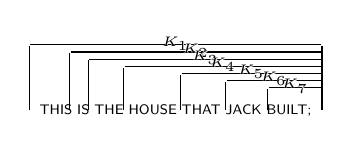
\begin{tikzpicture}[
    			>={Stealth[inset=0pt,length=4pt, angle'=45,round]},
    			word/.style = { font = \fontsize{5.25pt}{5.5pt}\selectfont, inner sep=0.1pt, outer sep=0.1pt, text = black },
    			fake/.style = { inner sep=0pt, outer sep=0pt },
			]
			
			\def\oneUnit{0.6cm}
			\def\customFontSize{4pt}
			
			\node[word] (zawartoscPliku) at (0*\oneUnit, 0*\oneUnit) {THIS IS THE HOUSE THAT JACK BUILT;};
			
			\node[fake] (koniecZawartosciPliku) at (3.1*\oneUnit, 0*\oneUnit) {};
			\node[fake] (poczatekZawartosciPliku) at (-3.1*\oneUnit, 0*\oneUnit) {};
			
			\node[fake] (nadPoczatkiemZawartosciPliku) at (-3.1*\oneUnit, 1.4*\oneUnit) {};
			
			\node[fake] (nadKoncemZawartosciPliku1) at (3.1*\oneUnit, 1.4*\oneUnit) {};
			\node[fake] (nadKoncemZawartosciPliku2) at (3.1*\oneUnit, 1.25*\oneUnit) {};
			\node[fake] (nadKoncemZawartosciPliku3) at (3.1*\oneUnit, 1.1*\oneUnit) {};
			\node[fake] (nadKoncemZawartosciPliku4) at (3.1*\oneUnit, 0.95*\oneUnit) {};
			\node[fake] (nadKoncemZawartosciPliku5) at (3.1*\oneUnit, 0.8*\oneUnit) {};
			\node[fake] (nadKoncemZawartosciPliku6) at (3.1*\oneUnit, 0.65*\oneUnit) {};
			\node[fake] (nadKoncemZawartosciPliku7) at (3.1*\oneUnit, 0.5*\oneUnit) {};
			
			\node[fake] (koniecThis) at (-2.25*\oneUnit, 0*\oneUnit) {};
			
			\node[fake] (nadKoniecThis1) at (-2.25*\oneUnit, 1.25*\oneUnit) {};
			
			\node[fake] (koniecIs) at (-1.85*\oneUnit, 0*\oneUnit) {};
			
			\node[fake] (nadKoniecIs1) at (-1.85*\oneUnit, 1.1*\oneUnit) {};
			
			\node[fake] (koniecThe) at (-1.1*\oneUnit, 0*\oneUnit) {};
			
			\node[fake] (nadKoniecThe1) at (-1.1*\oneUnit, 0.95*\oneUnit) {};
			
			\node[fake] (koniecHouse) at (0.1*\oneUnit, 0*\oneUnit) {};
			
			\node[fake] (nadKoniecHouse1) at (0.1*\oneUnit, 0.8*\oneUnit) {};
			
			\node[fake] (koniecThat) at (1.05*\oneUnit, 0*\oneUnit) {};
			
			\node[fake] (nadKoniecThat1) at (1.05*\oneUnit, 0.65*\oneUnit) {};
			
			\node[fake] (koniecJack) at (1.95*\oneUnit, 0*\oneUnit) {};
			
			\node[fake] (nadKoniecJack1) at (1.95*\oneUnit, 0.5*\oneUnit) {};
			
			\path (poczatekZawartosciPliku) edge [] (nadPoczatkiemZawartosciPliku);
			
			\path (koniecThis) edge [] (nadKoniecThis1);
			
			\path (koniecIs) edge [] (nadKoniecIs1);
			
			\path (koniecThe) edge [] (nadKoniecThe1);
			
			\path (koniecThe) edge [] (nadKoniecThe1);
			
			\path (koniecHouse) edge [] (nadKoniecHouse1);
			
			\path (koniecThat) edge [] (nadKoniecThat1);
			
			\path (koniecJack) edge [] (nadKoniecJack1);
			
			\path (koniecZawartosciPliku) edge [] (nadKoncemZawartosciPliku1);
			\path (koniecZawartosciPliku) edge [] (nadKoncemZawartosciPliku2);
			\path (koniecZawartosciPliku) edge [] (nadKoncemZawartosciPliku3);
			\path (koniecZawartosciPliku) edge [] (nadKoncemZawartosciPliku4);
			\path (koniecZawartosciPliku) edge [] (nadKoncemZawartosciPliku5);
			\path (koniecZawartosciPliku) edge [] (nadKoncemZawartosciPliku6);
			\path (koniecZawartosciPliku) edge [] (nadKoncemZawartosciPliku7);
			
			\path (nadPoczatkiemZawartosciPliku) edge [] node[above = -0.325*\oneUnit] {\fontsize{\customFontSize}{\customFontSize}\selectfont \contour{white}{$K_1$}} (nadKoncemZawartosciPliku1);
			\path (nadKoniecThis1) edge [] node[above = -0.325*\oneUnit] {\fontsize{\customFontSize}{\customFontSize}\selectfont \contour{white}{$K_2$}} (nadKoncemZawartosciPliku2);
			\path (nadKoniecIs1) edge [] node[above = -0.325*\oneUnit] {\fontsize{\customFontSize}{\customFontSize}\selectfont \contour{white}{$K_3$}} (nadKoncemZawartosciPliku3);
			\path (nadKoniecThe1) edge [] node[above = -0.325*\oneUnit] {\fontsize{\customFontSize}{\customFontSize}\selectfont \contour{white}{$K_4$}} (nadKoncemZawartosciPliku4);
			\path (nadKoniecHouse1) edge [] node[above = -0.325*\oneUnit] {\fontsize{\customFontSize}{\customFontSize}\selectfont \contour{white}{$K_5$}} (nadKoncemZawartosciPliku5);
			\path (nadKoniecThat1) edge [] node[above = -0.325*\oneUnit] {\fontsize{\customFontSize}{\customFontSize}\selectfont \contour{white}{$K_6$}} (nadKoncemZawartosciPliku6);
			\path (nadKoniecJack1) edge [] node[above = -0.325*\oneUnit] {\fontsize{\customFontSize}{\customFontSize}\selectfont \contour{white}{$K_7$}} (nadKoncemZawartosciPliku7);
        			\end{tikzpicture}
        		\end{figure}%
%%%%%%%%%%%%%%%%%%%%%%%%%%%%%%%%%%%%%%%%%%%%%%%%%%%%%%%%%%%%%%%%%%%%%%%%%%%%%%%%%%%%%%%%%%%%%%%%%%%%%%%%%%%%%%%%%%%%%%%%%%%%%%%%%%%%%%%%%%%%%%%%%%%%%%%%%%%%%%%%%%%%%%%%%%%%%%%%%%%%%%%%%%%%%%%%%%%%%%%%%%%%%%%%%%%%%%%%%%%%%%%%%%%%%%%%%%%%%%%%%%%%%%%%%%%%%%%%%%%%%%%%%%%%%%%%%%%%%%%%%%%%%%%%%%%%%%%%%%%%%%%%%%%%%%%%%%%%%%%%%%%%%
\contourlength{2.5pt}%
%%%%%%%%%%%%%%%%%%%%%%%%%%%%%%%%%%%%%%%%%%%%%%%%%%%%%%%%%%%%%%%%%%%%%%%%%%%%%%%%%%%%%%%%%%%%%%%%%%%%%%%%%%%%%%%%%%%%%%%%%%%%%%%%%%%%%%%%%%%%%%%%%%%%%%%%%%%%%%%%%%%%%%%%%%%%%%%%%%%%%%%%%%%%%%%%%%%%%%%%%%%%%%%%%%%%%%%%%%%%%%%%%%%%%%%%%%%%%%%%%%%%%%%%%%%%%%%%%%%%%%%%%%%%%%%%%%%%%%%%%%%%%%%%%%%%%%%%%%%%%%%%%%%%%%%%%%%%%%%%%%%%%
	        \column{0.4\textwidth}
\vspace*{-0.6cm}%
    	        \begin{figure}[H]
            	       % \caption{Drzewo Patricia}\label{fig:DrzewoPatricia}
                	    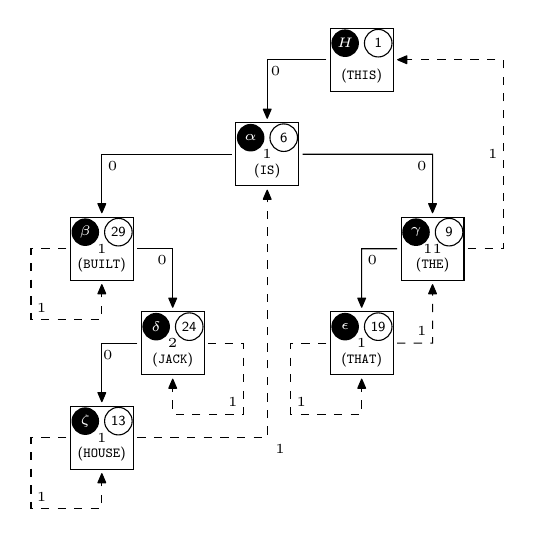
\begin{tikzpicture}[
                    	    >={Stealth[inset=0pt,length=4pt, angle'=45,round]},
        		nodeBox/.style = { rectangle, top color = white, bottom color = white, draw, black, text = black, minimum width = 0.8 cm, minimum height = 0.8 cm, font = \tiny, inner sep=0.05cm, outer sep=0.05cm },
        		word/.style = { font = \tiny, inner sep=0.5pt, outer sep=0.5pt, text = black },
        		greekSymbol/.style = { ellipse, minimum width = 0.35 cm, minimum height = 0.35 cm, fill, color = black, font = \tiny, inner sep=0pt, outer sep = 0pt, text = white },
        		position/.style = { ellipse, minimum width = 0.35 cm, minimum height = 0.35 cm, top color = white, bottom color = white, draw, black, font = \tiny, inner sep=0pt, outer sep = 0pt, text = black},
        		        ]
        \def\oneUnit{0.6cm}
		
		\node[nodeBox] (THISskip) at (-2*\oneUnit,1*\oneUnit) {};
		\node[greekSymbol] (THISsymbol) at (-2.35*\oneUnit, 1.35*\oneUnit) {$H$};
		\node[position] (THISposition) at (-1.65*\oneUnit, 1.35*\oneUnit) {1};
		\node[word] (THIS) at (-2*\oneUnit, 0.65*\oneUnit) {(\texttt{THIS})};
		
		
		
		\node[nodeBox] (ISskip) at (-4*\oneUnit,-1*\oneUnit) {$1$};
		\node[greekSymbol] (ISsymbol) at (-4.35*\oneUnit, -0.65*\oneUnit) {$\alpha$};
		\node[position] (ISposition) at (-3.65*\oneUnit,-0.65*\oneUnit) {6};
		\node[word] (IS) at (-4*\oneUnit, -1.35*\oneUnit) {(\texttt{IS})};
		
		
		
		\node[nodeBox] (BUILTskip) at (-7.5*\oneUnit,-3*\oneUnit) {$1$};
		\node[greekSymbol] (BUILTsymbol) at (-7.85*\oneUnit, -2.65*\oneUnit) {$\beta$};
		\node[position] (BUILTposition) at (-7.15*\oneUnit,-2.65*\oneUnit) {29};
		\node[word] (BUILT) at (-7.5*\oneUnit, -3.35*\oneUnit) {(\texttt{BUILT})};
		
		\node[nodeBox] (THEskip) at (-0.5*\oneUnit,-3*\oneUnit) {$11$};
		\node[greekSymbol] (THEsymbol) at (-0.85*\oneUnit, -2.65*\oneUnit) {$\gamma$};
		\node[position] (THEposition) at (-0.15*\oneUnit,-2.65*\oneUnit) {9};
		\node[word] (THE) at (-0.5*\oneUnit, -3.35*\oneUnit) {(\texttt{THE})};
		
		
		
		\node[nodeBox] (JACKskip) at (-6*\oneUnit,-5*\oneUnit) {$2$};
		\node[greekSymbol] (JACKsymbol) at (-6.35*\oneUnit, -4.65*\oneUnit) {$\delta$};
		\node[position] (JACKposition) at (-5.65*\oneUnit,-4.65*\oneUnit) {24};
		\node[word] (JACK) at (-6*\oneUnit, -5.35*\oneUnit) {(\texttt{JACK})};
		
		\node[nodeBox] (THATskip) at (-2*\oneUnit,-5*\oneUnit) {$1$};
		\node[greekSymbol] (THATsymbol) at (-2.35*\oneUnit, -4.65*\oneUnit) {$\epsilon$};
		\node[position] (THATposition) at (-1.65*\oneUnit,-4.65*\oneUnit) {19};
		\node[word] (THAT) at (-2*\oneUnit, -5.35*\oneUnit) {(\texttt{THAT})};
		
		
		
		\node[nodeBox] (HOUSEskip) at (-7.5*\oneUnit,-7*\oneUnit) {$1$};
		\node[greekSymbol] (HOUSEsymbol) at (-7.85*\oneUnit, -6.65*\oneUnit) {$\zeta$};
		\node[position] (HOUSEposition) at (-7.15*\oneUnit,-6.65*\oneUnit) {13};
		\node[word] (HOUSE) at (-7.5*\oneUnit, -7.35*\oneUnit) {(\texttt{HOUSE})};
		
		\draw [->] (THISskip) -- node[yshift = -0.25*\oneUnit, xshift = -0.45*\oneUnit] {\tiny $0$} ++ (-2*\oneUnit, 0*\oneUnit) -- (ISskip);
		
		\draw [->] (ISskip) -- node[yshift = -0.25*\oneUnit, xshift = -1.15*\oneUnit] {\tiny $0$} ++ (-3.5*\oneUnit, 0*\oneUnit) -- (BUILTskip);
		\draw [->] (ISskip) -- node[yshift = -0.25*\oneUnit, xshift = 1.15*\oneUnit] {\tiny $0$} ++ (3.5*\oneUnit, 0*\oneUnit) -- (THEskip);
		
		\draw [->, dashed] (BUILTskip) -- node[yshift = -1.25*\oneUnit, xshift = -0.15*\oneUnit] {\tiny $1$} ++(-1.5*\oneUnit, 0*\oneUnit) -- ++(0*\oneUnit, -1.5*\oneUnit) -- ++(1.5*\oneUnit, 0*\oneUnit) -- (BUILTskip);
		\draw [->] (BUILTskip) -- node[yshift = -0.25*\oneUnit, xshift = 0.15*\oneUnit] {\tiny $0$} ++(1.5*\oneUnit, 0*\oneUnit) -- (JACKskip);
		
		\draw [->] (THEskip) -- node[yshift = -0.25*\oneUnit, xshift = -0.15*\oneUnit] {\tiny $0$} ++(-1.5*\oneUnit, 0*\oneUnit) -- (THATskip);
		\draw [->, dashed] (THEskip) -- node[yshift = 2.0*\oneUnit, xshift = 0.15*\oneUnit] {\tiny $1$} ++ (1.5*\oneUnit, 0*\oneUnit) -- ++ (0*\oneUnit, 4*\oneUnit) -- (THISskip);
		
		
		\draw [->, dashed] (THATskip) -- node[yshift = -1.25*\oneUnit, xshift = -0.15*\oneUnit] {\tiny $1$} ++(-1.5*\oneUnit, 0*\oneUnit) -- ++(0*\oneUnit, -1.5*\oneUnit) -- ++(1.5*\oneUnit, 0*\oneUnit) -- (THATskip);
		\draw [->, dashed] (THATskip) -- node[yshift = 0.25*\oneUnit, xshift = 0.15*\oneUnit] {\tiny $1$} ++ (1.5*\oneUnit, 0*\oneUnit) -- (THEskip);
		
		\draw [->] (JACKskip) -- node[yshift = -0.25*\oneUnit, xshift = -0.25*\oneUnit] {\tiny $0$} ++(-1.5*\oneUnit, 0*\oneUnit) -- (HOUSEskip);
		\draw [->, dashed] (JACKskip) -- node[yshift = -1.25*\oneUnit, xshift = 0.15*\oneUnit] {\tiny $1$} ++(1.5*\oneUnit, 0*\oneUnit) -- ++(0*\oneUnit, -1.5*\oneUnit) -- ++(-1.5*\oneUnit, 0*\oneUnit) -- (JACKskip);
		
		\draw [->, dashed] (HOUSEskip) -- node[yshift = -1.25*\oneUnit, xshift = -0.15*\oneUnit] {\tiny $1$} ++(-1.5*\oneUnit, 0*\oneUnit) -- ++(0*\oneUnit, -1.5*\oneUnit) -- ++(1.5*\oneUnit, 0*\oneUnit) -- (HOUSEskip);
		\draw [->, dashed] (HOUSEskip) -- node[yshift = -0.25*\oneUnit, xshift = 1.65*\oneUnit] {\tiny $1$} ++(3.5*\oneUnit, 0*\oneUnit) -- (ISskip);
		\end{tikzpicture}
        		        
        		\end{figure}
    	\end{columns}
    \end{frame}
    %%%%%%%%%%%%%%%%%%%%%%%%%%%
  	\section{Autorski program - Zrealizowana implementacja}
	%%%%%%%%%%%%%%%%%%%%%%%%%%%
	\begin{frame}{Drzewo \emph{Patricia}}{Implementacja na podstawie algorytmów Knuth'a}
	    Implementacja mojego programu w języku \emph{Java} zawiera:
	    \begin{enumerate}
	        \item {\color{AGH@green} Implementację funkcjonalności drzewa \emph{Patricia}}:
            \begin{enumerate}
                \item {\color{AGH@green} Operacje:}
                \begin{enumerate}
                    \item {\color{AGH@green} Wstawienie nowego \textbf{KLUCZA}} {\color{gray} (z istniejącego pliku źródłowego)}. \newline 
                    {\scriptsize \color{gray} \hspace*{0.4cm} - Insert \textbf{KEY} \color{lightgray} (From Existing File)}
                    
                    \item Przeszukiwania względem \textbf{PREFIKSÓW}:
                    
                        \setcounter{enumiii}{0}
                        \addtolength{\itemindent}{0.7cm}
                        \item {\color{AGH@green} Czy drzewo zawiera słowo $X$ jako \textbf{PREFIKS}?} \newline 
                        {\scriptsize \color{gray} \hspace*{0.4cm} - Look-up \textbf{PREFIX}}
                        
                        \item {\color{AGH@green} Które węzły akceptują słowo $X$ jako \textbf{PREFIKS}?} \newline 
                        {\scriptsize \color{gray} \hspace*{0.4cm} - Search \textbf{PREFIX}} 
                \end{enumerate}
                
                \hspace*{-1.65cm} Na podstawie 3 algorytmów przeznaczonych na Maszynę MIX Knuth'a, której bajt ma 5 bitów \newline
                
                \item {\color{AGH@green} Symulacje Maszyny MIX}
                \begin{enumerate}
                    \color{gray}
                    \item o parametryzowanej ilości bitów w bajcie \newline
                    \hspace{0.45cm} {\color{lightgray} (od 5 wzwyż, zwykle bajt maszyny MIX ma 6 bitów)}
                    \item oraz tablicy kodowania znaków \newline
                    \hspace{0.45cm} {\color{lightgray} (aby zapewnić obsługę wymaganych znaków w odpowiednim zakresie liczbowym)}.
                \end{enumerate}
            \end{enumerate}
	    \end{enumerate}
	\end{frame}	
  	%%%%%%%%%%%%%%%%%%%%%%%%%%%
	\begin{frame}{Drzewo \emph{Patricia}}{Autorskie rozszerzenie na podstawie wcześniejszej implementacji}
	    \hspace*{-0.6cm}{\color{AGH@green}Implementacja dodatkowych funkcjonalności autorskich} drzewa \emph{Patrcia} 
        \begin{enumerate}
            \addtolength{\itemindent}{-0.6cm}
            \item {\color{AGH@green}Strategia klucza (2)} definiująca go w postaci pojedynczego słowa - rozłącznych kluczy
            \item {\color{AGH@green}Operacje:} 
            \begin{enumerate}
                \addtolength{\itemindent}{-0.6cm}
                \item {\color{AGH@green} Wstawienie wszystkich \textbf{KLUCZY}} {\color{gray} (z istniejącego pliku źródłowego)} \newline 
                    {\scriptsize \color{gray} \hspace*{0.4cm} - Insert All \textbf{KEYS} \color{lightgray} (From Existing File)}
                
                \item Przeszukiwania względem \textbf{KLUCZY}:
                
                    \setcounter{enumii}{0}
                    \addtolength{\itemindent}{0.7cm}
                    \item {\color{AGH@green} Czy drzewo zawiera słowo $X$ jako \textbf{KLUCZ}?} \newline 
                        {\scriptsize \color{gray} \hspace*{0.4cm} - Look-up \textbf{KEY}}
                    \item {\color{AGH@green} Który węzeł akceptuje słowo $X$ jako \textbf{KLUCZ}?} \newline 
                        {\scriptsize \color{gray} \hspace*{0.4cm} - Search \textbf{KEY}} \newline
            \end{enumerate}
        \end{enumerate}
        
        \hspace*{-0.6cm} Na podstawie wcześniej \newline
        \hspace*{-0.6cm} zaimplementowanych funkcjonalności
%%%%%%%%%%%%%%%%%%%%%%%%%%%%%%%%%%%%%%%%%%%%%%%%%%%%%%%%%%%%%%%%%%%%%%%%%%%%%%%%%%%%%%%%%%%%%%%%%%%%%%%%%%%%%%%%%%%%%%%%%%%%%%%%%%%%%%%%%%%%%%%%%%%%%%%%%%%%%%%%%%%%%%%%%%%%%%%%%%%%%%%%%%%%%%%%%%%%%%%%%%%%%%%%%%%%%%%%%%%%%%%%%%%%%%%%%%%%%%%%%%%%%%%%%%%%%%%%%%%%%%%%%%%%%%%%%%%%%%%%%%%%%%%%%%%%%%%%%%%%%%%%%%%%%%%%%%%%%%%%%%%%%
\contourlength{0.5pt}%
%%%%%%%%%%%%%%%%%%%%%%%%%%%%%%%%%%%%%%%%%%%%%%%%%%%%%%%%%%%%%%%%%%%%%%%%%%%%%%%%%%%%%%%%%%%%%%%%%%%%%%%%%%%%%%%%%%%%%%%%%%%%%%%%%%%%%%%%%%%%%%%%%%%%%%%%%%%%%%%%%%%%%%%%%%%%%%%%%%%%%%%%%%%%%%%%%%%%%%%%%%%%%%%%%%%%%%%%%%%%%%%%%%%%%%%%%%%%%%%%%%%%%%%%%%%%%%%%%%%%%%%%%%%%%%%%%%%%%%%%%%%%%%%%%%%%%%%%%%%%%%%%%%%%%%%%%%%%%%%%%%%%%
	    		 \vspace*{-4.05cm} \begin{figure}
			\centering \hspace*{8.5cm}
			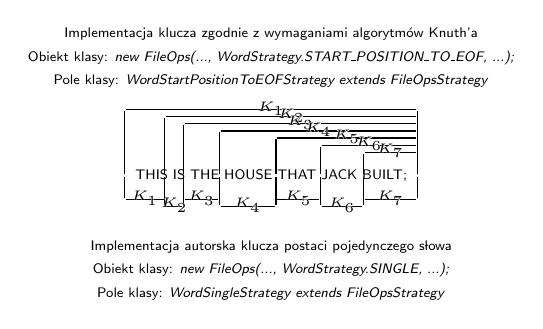
\begin{tikzpicture}[
    			>={Stealth[inset=0pt,length=4pt, angle'=45,round]},
    			word/.style = { font = \fontsize{5.25pt}{5.5pt}\selectfont, inner sep=0.1pt, outer sep=0.1pt, text = black },
    			fake/.style = { inner sep=0pt, outer sep=0pt },
			]
			
			\def\oneUnit{0.6cm}
			\def\customFontSize{4pt}
			
			\node[word] (zawartoscPliku) at (0*\oneUnit, 0*\oneUnit) {THIS IS THE HOUSE THAT JACK BUILT;};
			
			\node[word] (wordStartPositionToEOFStrategy) at (0*\oneUnit, 2*\oneUnit) {Pole klasy: \emph{WordStartPositionToEOFStrategy extends FileOpsStrategy}};
			\node[word] (wordSingleStrategy) at (0*\oneUnit, -2.5*\oneUnit) {Pole klasy: \emph{WordSingleStrategy extends FileOpsStrategy}};
			
			
			\node[word] (fileOpsSPTEOF) at (0*\oneUnit, 2.5*\oneUnit) {Obiekt klasy: \emph{new FileOps(..., WordStrategy.START\textunderscore POSITION\textunderscore TO\textunderscore EOF, ...);}};
			\node[word] (fileOpsSingle) at (0*\oneUnit, -2*\oneUnit) {Obiekt klasy: \emph{new FileOps(..., WordStrategy.SINGLE, ...);}};
			
			\node[word] (implementacjaKnuth) at (0*\oneUnit, 3*\oneUnit) {Implementacja klucza zgodnie z wymaganiami algorytmów Knuth'a};
			\node[word] (implementacjaAutorska) at (0*\oneUnit, -1.5*\oneUnit) {Implementacja autorska klucza postaci pojedynczego słowa};
			
			\node[fake] (koniecZawartosciPliku) at (3.1*\oneUnit, 0*\oneUnit) {};
			\node[fake] (poczatekZawartosciPliku) at (-3.1*\oneUnit, 0*\oneUnit) {};
			
			\node[fake] (nadPoczatkiemZawartosciPliku) at (-3.1*\oneUnit, 1.4*\oneUnit) {};
			\node[fake] (podPoczatkiemZawartosciPliku) at (-3.1*\oneUnit, -0.5*\oneUnit) {};
			
			\node[fake] (nadKoncemZawartosciPliku1) at (3.1*\oneUnit, 1.4*\oneUnit) {};
			\node[fake] (nadKoncemZawartosciPliku2) at (3.1*\oneUnit, 1.25*\oneUnit) {};
			\node[fake] (nadKoncemZawartosciPliku3) at (3.1*\oneUnit, 1.1*\oneUnit) {};
			\node[fake] (nadKoncemZawartosciPliku4) at (3.1*\oneUnit, 0.95*\oneUnit) {};
			\node[fake] (nadKoncemZawartosciPliku5) at (3.1*\oneUnit, 0.8*\oneUnit) {};
			\node[fake] (nadKoncemZawartosciPliku6) at (3.1*\oneUnit, 0.65*\oneUnit) {};
			\node[fake] (nadKoncemZawartosciPliku7) at (3.1*\oneUnit, 0.5*\oneUnit) {};
			
			\node[fake] (podKoncemZawartosciPliku1) at (3.1*\oneUnit, -0.5*\oneUnit) {};
			
			\node[fake] (koniecThis) at (-2.25*\oneUnit, 0*\oneUnit) {};
			
			\node[fake] (nadKoniecThis1) at (-2.25*\oneUnit, 1.25*\oneUnit) {};
			\node[fake] (podKoniecThis1) at (-2.25*\oneUnit, -0.5*\oneUnit) {};
			
			\node[fake] (podKoniecThis2) at (-2.25*\oneUnit, -0.65*\oneUnit) {};
			
			\node[fake] (koniecIs) at (-1.85*\oneUnit, 0*\oneUnit) {};
			
			\node[fake] (nadKoniecIs1) at (-1.85*\oneUnit, 1.1*\oneUnit) {};
			\node[fake] (podKoniecIs1) at (-1.85*\oneUnit, -0.5*\oneUnit) {};
			
			\node[fake] (podKoniecIs2) at (-1.85*\oneUnit, -0.65*\oneUnit) {};
			
			\node[fake] (koniecThe) at (-1.1*\oneUnit, 0*\oneUnit) {};
			
			\node[fake] (nadKoniecThe1) at (-1.1*\oneUnit, 0.95*\oneUnit) {};
			\node[fake] (podKoniecThe1) at (-1.1*\oneUnit, -0.5*\oneUnit) {};
			
			\node[fake] (podKoniecThe2) at (-1.1*\oneUnit, -0.65*\oneUnit) {};
			
			\node[fake] (koniecHouse) at (0.1*\oneUnit, 0*\oneUnit) {};
			
			\node[fake] (nadKoniecHouse1) at (0.1*\oneUnit, 0.8*\oneUnit) {};
			\node[fake] (podKoniecHouse1) at (0.1*\oneUnit, -0.5*\oneUnit) {};
			
			\node[fake] (podKoniecHouse2) at (0.1*\oneUnit, -0.65*\oneUnit) {};
			
			\node[fake] (koniecThat) at (1.05*\oneUnit, 0*\oneUnit) {};
			
			\node[fake] (nadKoniecThat1) at (1.05*\oneUnit, 0.65*\oneUnit) {};
			\node[fake] (podKoniecThat1) at (1.05*\oneUnit, -0.5*\oneUnit) {};
			
			\node[fake] (podKoniecThat2) at (1.05*\oneUnit, -0.65*\oneUnit) {};
			
			\node[fake] (koniecJack) at (1.95*\oneUnit, 0*\oneUnit) {};
			
			\node[fake] (nadKoniecJack1) at (1.95*\oneUnit, 0.5*\oneUnit) {};
			\node[fake] (podKoniecJack1) at (1.95*\oneUnit, -0.5*\oneUnit) {};
			
			\node[fake] (podKoniecJack2) at (1.95*\oneUnit, -0.65*\oneUnit) {};
			
			\path (poczatekZawartosciPliku) edge [] (nadPoczatkiemZawartosciPliku);
			\path (poczatekZawartosciPliku) edge [] (podPoczatkiemZawartosciPliku);
			
			\path (koniecThis) edge [] (nadKoniecThis1);
			\path (koniecThis) edge [] (podKoniecThis1);
			
			\path (koniecThis) edge [] (podKoniecThis2);
			
			\path (koniecIs) edge [] (nadKoniecIs1);
			\path (koniecIs) edge [] (podKoniecIs1);
			
			\path (koniecIs) edge [] (podKoniecIs2);
			
			\path (koniecThe) edge [] (nadKoniecThe1);
			\path (koniecThe) edge [] (podKoniecThe2);
			
			\path (koniecThe) edge [] (nadKoniecThe1);
			\path (koniecThe) edge [] (podKoniecThe2);
			
			\path (koniecHouse) edge [] (nadKoniecHouse1);
			\path (koniecHouse) edge [] (podKoniecHouse1);
			
			\path (koniecHouse) edge [] (podKoniecHouse2);
			
			\path (koniecThat) edge [] (nadKoniecThat1);
			\path (koniecThat) edge [] (podKoniecThat1);
			
			\path (koniecThat) edge [] (podKoniecThat2);
			
			\path (koniecJack) edge [] (nadKoniecJack1);
			\path (koniecJack) edge [] (podKoniecJack1);
			
			\path (koniecJack) edge [] (podKoniecJack2);
			
			\path (koniecZawartosciPliku) edge [] (nadKoncemZawartosciPliku1);
			\path (koniecZawartosciPliku) edge [] (nadKoncemZawartosciPliku2);
			\path (koniecZawartosciPliku) edge [] (nadKoncemZawartosciPliku3);
			\path (koniecZawartosciPliku) edge [] (nadKoncemZawartosciPliku4);
			\path (koniecZawartosciPliku) edge [] (nadKoncemZawartosciPliku5);
			\path (koniecZawartosciPliku) edge [] (nadKoncemZawartosciPliku6);
			\path (koniecZawartosciPliku) edge [] (nadKoncemZawartosciPliku7);
			
			\path (koniecZawartosciPliku) edge [] (podKoncemZawartosciPliku1);
			
			\path (nadPoczatkiemZawartosciPliku) edge [] node[above = -0.325*\oneUnit] {\fontsize{\customFontSize}{\customFontSize}\selectfont \contour{white}{$K_1$}} (nadKoncemZawartosciPliku1);
			\path (nadKoniecThis1) edge [] node[above = -0.325*\oneUnit] {\fontsize{\customFontSize}{\customFontSize}\selectfont \contour{white}{$K_2$}} (nadKoncemZawartosciPliku2);
			\path (nadKoniecIs1) edge [] node[above = -0.325*\oneUnit] {\fontsize{\customFontSize}{\customFontSize}\selectfont \contour{white}{$K_3$}} (nadKoncemZawartosciPliku3);
			\path (nadKoniecThe1) edge [] node[above = -0.325*\oneUnit] {\fontsize{\customFontSize}{\customFontSize}\selectfont \contour{white}{$K_4$}} (nadKoncemZawartosciPliku4);
			\path (nadKoniecHouse1) edge [] node[above = -0.325*\oneUnit] {\fontsize{\customFontSize}{\customFontSize}\selectfont \contour{white}{$K_5$}} (nadKoncemZawartosciPliku5);
			\path (nadKoniecThat1) edge [] node[above = -0.325*\oneUnit] {\fontsize{\customFontSize}{\customFontSize}\selectfont \contour{white}{$K_6$}} (nadKoncemZawartosciPliku6);
			\path (nadKoniecJack1) edge [] node[above = -0.325*\oneUnit] {\fontsize{\customFontSize}{\customFontSize}\selectfont \contour{white}{$K_7$}} (nadKoncemZawartosciPliku7);
			
			\path (podPoczatkiemZawartosciPliku) edge [] node[above = -0.325*\oneUnit] {\fontsize{\customFontSize}{\customFontSize}\selectfont \contour{white}{$K_1$}} (podKoniecThis1);
			\path (podKoniecThis2) edge [] node[above = -0.325*\oneUnit] {\fontsize{\customFontSize}{\customFontSize}\selectfont \contour{white}{$K_2$}} (podKoniecIs2);
			\path (podKoniecIs1) edge [] node[above = -0.325*\oneUnit] {\fontsize{\customFontSize}{\customFontSize}\selectfont \contour{white}{$K_3$}} (podKoniecThe1);
			\path (podKoniecThe2) edge [] node[above = -0.325*\oneUnit] {\fontsize{\customFontSize}{\customFontSize}\selectfont \contour{white}{$K_4$}} (podKoniecHouse2);
			\path (podKoniecHouse1) edge [] node[above = -0.325*\oneUnit] {\fontsize{\customFontSize}{\customFontSize}\selectfont \contour{white}{$K_5$}} (podKoniecThat1);
			\path (podKoniecThat2) edge [] node[above = -0.325*\oneUnit] {\fontsize{\customFontSize}{\customFontSize}\selectfont \contour{white}{$K_6$}} (podKoniecJack2);
			\path (podKoniecJack1) edge [] node[above = -0.325*\oneUnit] {\fontsize{\customFontSize}{\customFontSize}\selectfont \contour{white}{$K_7$}} (podKoncemZawartosciPliku1);
			
			\end{tikzpicture}
		        \end{figure}%
%%%%%%%%%%%%%%%%%%%%%%%%%%%%%%%%%%%%%%%%%%%%%%%%%%%%%%%%%%%%%%%%%%%%%%%%%%%%%%%%%%%%%%%%%%%%%%%%%%%%%%%%%%%%%%%%%%%%%%%%%%%%%%%%%%%%%%%%%%%%%%%%%%%%%%%%%%%%%%%%%%%%%%%%%%%%%%%%%%%%%%%%%%%%%%%%%%%%%%%%%%%%%%%%%%%%%%%%%%%%%%%%%%%%%%%%%%%%%%%%%%%%%%%%%%%%%%%%%%%%%%%%%%%%%%%%%%%%%%%%%%%%%%%%%%%%%%%%%%%%%%%%%%%%%%%%%%%%%%%%%%%%%
\contourlength{2.5pt}%
%%%%%%%%%%%%%%%%%%%%%%%%%%%%%%%%%%%%%%%%%%%%%%%%%%%%%%%%%%%%%%%%%%%%%%%%%%%%%%%%%%%%%%%%%%%%%%%%%%%%%%%%%%%%%%%%%%%%%%%%%%%%%%%%%%%%%%%%%%%%%%%%%%%%%%%%%%%%%%%%%%%%%%%%%%%%%%%%%%%%%%%%%%%%%%%%%%%%%%%%%%%%%%%%%%%%%%%%%%%%%%%%%%%%%%%%%%%%%%%%%%%%%%%%%%%%%%%%%%%%%%%%%%%%%%%%%%%%%%%%%%%%%%%%%%%%%%%%%%%%%%%%%%%%%%%%%%%%%%%%%%%%%
	\end{frame}	
	%%%%%%%%%%%%%%%%%%%%%%%%%%%
	\begin{frame}{Konwerter DIMACS CNF}{Autorska implementacja konwertera na pliki źródłowe implementacji drzewa \emph{Patricia}}
	\scriptsize
	{\color{AGH@green}CNF} – koniunkcyjna postać normalna – formuła logiczna postaci koniunkcji klauzul. 
	
    {\color{AGH@green}DIMACS CNF} – format zapisu plików CNF.
    
    {\color{AGH@green}Konwerter} sortuje literały wewnątrz każdej z klauzul oraz zapisuje je w nowym pliku. \newline 
        \hspace*{0.76cm}Nowy plik jest parametryzowany względem znaków rozdzielających literały, klauzule, koniec pliku. \newline
	    {   \color{gray}\tiny
	        \hspace*{0.76cm} Implementacja konwertera plików DIMACS CNF na pliki źródłowe drzewa \emph{Patricia}. \newline
	        {   \color{gray}\tiny
	            \hspace*{1.25cm} Bez linii tekstu niezawierających kluczowych informacji \newline 
	                \hspace*{1.75cm} {\color{lightgray} - O klauzulach w koniunkcyjnej postaci normalnej - (linii komentarzy i problemu),} \newline 
	            \hspace*{1.25cm} O posortowanych literałach wewnątrz każdej z klauzul, \newline 
	            \hspace*{1.25cm} Ze zmodyfikowanymi parametryzowanymi znakami rozdzielającymi literały wewnątrz klauzul oraz same klauzule \newline
	            \hspace*{1.25cm} i o dodanym parametryzowanym znaku końca pliku.
	        }
	    }
	    \vspace*{-0.1cm}
	    \begin{columns}
	        \column{0.15\textwidth}
	            \usebox\cnfBox \newline
	            
	            {\color{gray}\scriptsize CNF}
	        \column{0.21\textwidth}
	            \usebox\cnfIn \newline
	            
	            {\color{gray}\scriptsize DIMACS CNF}
	        \column{0.6\textwidth}
	            \usebox\cnfOut \newline
	            
	            {\color{gray}\scriptsize Plik źródłowy drzewa \emph{Patricia}}
	    \end{columns}
	\end{frame}	
  	%%%%%%%%%%%%%%%%%%%%%%%%%%%
	\begin{frame}{Reprezentacja graficzna 1.1}{Autorska implementacja samo-skalującej się reprezentacji struktury drzewa \emph{Patricia}}
        \vspace*{0.0cm}
	    \begin{columns}
	        \column{0.5\textwidth}
	            \centering
                \contour{white}{{\color{AGH@green}Rysunek:} Model}
	        \column{0.5\textwidth}
	            \centering
                \contour{white}{{\color{AGH@green}Rysunek:} Reprezentacja 1}
	    \end{columns}
    
        \begin{figure}[H]
            \fontsize{3}{5} \selectfont
            \vspace*{2.0cm}
            \hspace*{-5.7cm}
            \makebox[0pt][l]{%
                \raisebox{-\totalheight}[0pt][0pt]{%
                    \includegraphics[width=0.75\textwidth]{visaulRepresentation1.png}
                }
            }%
           % \includegraphics[width=1.15\textwidth]{visaulRepresentation1.png}
        \end{figure}
        
        \begin{figure}[H]
            \vspace*{-3.0cm}
	        \hspace*{-10cm}
    	    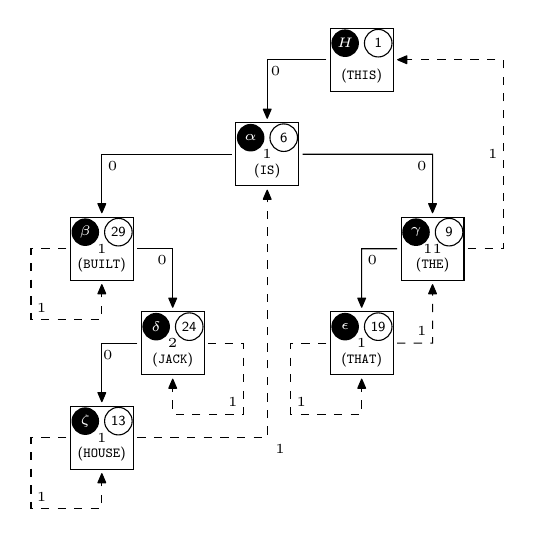
\begin{tikzpicture}[
        	    >={Stealth[inset=0pt,length=4pt, angle'=45,round]},
        		nodeBox/.style = { rectangle, top color = white, bottom color = white, draw, black, text = black, minimum width = 0.8 cm, minimum height = 0.8 cm, font = \tiny, inner sep=0.05cm, outer sep=0.05cm },
        		word/.style = { font = \tiny, inner sep=0.5pt, outer sep=0.5pt, text = black },
        		greekSymbol/.style = { ellipse, minimum width = 0.35 cm, minimum height = 0.35 cm, fill, color = black, font = \tiny, inner sep=0pt, outer sep = 0pt, text = white },
        		position/.style = { ellipse, minimum width = 0.35 cm, minimum height = 0.35 cm, top color = white, bottom color = white, draw, black, font = \tiny, inner sep=0pt, outer sep = 0pt, text = black},
	        ]
	        
                \def\oneUnit{0.6cm}
        		
        		\node[nodeBox] (THISskip) at (-2*\oneUnit,1*\oneUnit) {};
        		\node[greekSymbol] (THISsymbol) at (-2.35*\oneUnit, 1.35*\oneUnit) {$H$};
        		\node[position] (THISposition) at (-1.65*\oneUnit, 1.35*\oneUnit) {1};
        		\node[word] (THIS) at (-2*\oneUnit, 0.65*\oneUnit) {(\texttt{THIS})};
        		
        		
        		
        		\node[nodeBox] (ISskip) at (-4*\oneUnit,-1*\oneUnit) {$1$};
        		\node[greekSymbol] (ISsymbol) at (-4.35*\oneUnit, -0.65*\oneUnit) {$\alpha$};
        		\node[position] (ISposition) at (-3.65*\oneUnit,-0.65*\oneUnit) {6};
        		\node[word] (IS) at (-4*\oneUnit, -1.35*\oneUnit) {(\texttt{IS})};
        		
        		
        		
        		\node[nodeBox] (BUILTskip) at (-7.5*\oneUnit,-3*\oneUnit) {$1$};
        		\node[greekSymbol] (BUILTsymbol) at (-7.85*\oneUnit, -2.65*\oneUnit) {$\beta$};
        		\node[position] (BUILTposition) at (-7.15*\oneUnit,-2.65*\oneUnit) {29};
        		\node[word] (BUILT) at (-7.5*\oneUnit, -3.35*\oneUnit) {(\texttt{BUILT})};
        		
        		\node[nodeBox] (THEskip) at (-0.5*\oneUnit,-3*\oneUnit) {$11$};
        		\node[greekSymbol] (THEsymbol) at (-0.85*\oneUnit, -2.65*\oneUnit) {$\gamma$};
        		\node[position] (THEposition) at (-0.15*\oneUnit,-2.65*\oneUnit) {9};
        		\node[word] (THE) at (-0.5*\oneUnit, -3.35*\oneUnit) {(\texttt{THE})};
        		
        		
        		
        		\node[nodeBox] (JACKskip) at (-6*\oneUnit,-5*\oneUnit) {$2$};
        		\node[greekSymbol] (JACKsymbol) at (-6.35*\oneUnit, -4.65*\oneUnit) {$\delta$};
        		\node[position] (JACKposition) at (-5.65*\oneUnit,-4.65*\oneUnit) {24};
        		\node[word] (JACK) at (-6*\oneUnit, -5.35*\oneUnit) {(\texttt{JACK})};
        		
        		\node[nodeBox] (THATskip) at (-2*\oneUnit,-5*\oneUnit) {$1$};
        		\node[greekSymbol] (THATsymbol) at (-2.35*\oneUnit, -4.65*\oneUnit) {$\epsilon$};
        		\node[position] (THATposition) at (-1.65*\oneUnit,-4.65*\oneUnit) {19};
        		\node[word] (THAT) at (-2*\oneUnit, -5.35*\oneUnit) {(\texttt{THAT})};
        		
        		
        		
        		\node[nodeBox] (HOUSEskip) at (-7.5*\oneUnit,-7*\oneUnit) {$1$};
        		\node[greekSymbol] (HOUSEsymbol) at (-7.85*\oneUnit, -6.65*\oneUnit) {$\zeta$};
        		\node[position] (HOUSEposition) at (-7.15*\oneUnit,-6.65*\oneUnit) {13};
        		\node[word] (HOUSE) at (-7.5*\oneUnit, -7.35*\oneUnit) {(\texttt{HOUSE})};
        		
        		\draw [->] (THISskip) -- node[yshift = -0.25*\oneUnit, xshift = -0.45*\oneUnit] {\tiny $0$} ++ (-2*\oneUnit, 0*\oneUnit) -- (ISskip);
        		
        		\draw [->] (ISskip) -- node[yshift = -0.25*\oneUnit, xshift = -1.15*\oneUnit] {\tiny $0$} ++ (-3.5*\oneUnit, 0*\oneUnit) -- (BUILTskip);
        		\draw [->] (ISskip) -- node[yshift = -0.25*\oneUnit, xshift = 1.15*\oneUnit] {\tiny $0$} ++ (3.5*\oneUnit, 0*\oneUnit) -- (THEskip);
        		
        		\draw [->, dashed] (BUILTskip) -- node[yshift = -1.25*\oneUnit, xshift = -0.15*\oneUnit] {\tiny $1$} ++(-1.5*\oneUnit, 0*\oneUnit) -- ++(0*\oneUnit, -1.5*\oneUnit) -- ++(1.5*\oneUnit, 0*\oneUnit) -- (BUILTskip);
        		\draw [->] (BUILTskip) -- node[yshift = -0.25*\oneUnit, xshift = 0.15*\oneUnit] {\tiny $0$} ++(1.5*\oneUnit, 0*\oneUnit) -- (JACKskip);
        		
        		\draw [->] (THEskip) -- node[yshift = -0.25*\oneUnit, xshift = -0.15*\oneUnit] {\tiny $0$} ++(-1.5*\oneUnit, 0*\oneUnit) -- (THATskip);
        		\draw [->, dashed] (THEskip) -- node[yshift = 2.0*\oneUnit, xshift = 0.15*\oneUnit] {\tiny $1$} ++ (1.5*\oneUnit, 0*\oneUnit) -- ++ (0*\oneUnit, 4*\oneUnit) -- (THISskip);
        		
        		
        		\draw [->, dashed] (THATskip) -- node[yshift = -1.25*\oneUnit, xshift = -0.15*\oneUnit] {\tiny $1$} ++(-1.5*\oneUnit, 0*\oneUnit) -- ++(0*\oneUnit, -1.5*\oneUnit) -- ++(1.5*\oneUnit, 0*\oneUnit) -- (THATskip);
        		\draw [->, dashed] (THATskip) -- node[yshift = 0.25*\oneUnit, xshift = 0.15*\oneUnit] {\tiny $1$} ++ (1.5*\oneUnit, 0*\oneUnit) -- (THEskip);
        		
        		\draw [->] (JACKskip) -- node[yshift = -0.25*\oneUnit, xshift = -0.25*\oneUnit] {\tiny $0$} ++(-1.5*\oneUnit, 0*\oneUnit) -- (HOUSEskip);
        		\draw [->, dashed] (JACKskip) -- node[yshift = -1.25*\oneUnit, xshift = 0.15*\oneUnit] {\tiny $1$} ++(1.5*\oneUnit, 0*\oneUnit) -- ++(0*\oneUnit, -1.5*\oneUnit) -- ++(-1.5*\oneUnit, 0*\oneUnit) -- (JACKskip);
        		
        		\draw [->, dashed] (HOUSEskip) -- node[yshift = -1.25*\oneUnit, xshift = -0.15*\oneUnit] {\tiny $1$} ++(-1.5*\oneUnit, 0*\oneUnit) -- ++(0*\oneUnit, -1.5*\oneUnit) -- ++(1.5*\oneUnit, 0*\oneUnit) -- (HOUSEskip);
        		\draw [->, dashed] (HOUSEskip) -- node[yshift = -0.25*\oneUnit, xshift = 1.65*\oneUnit] {\tiny $1$} ++(3.5*\oneUnit, 0*\oneUnit) -- (ISskip);
        		
    		\end{tikzpicture}
        \end{figure}
	\end{frame}	
  	%%%%%%%%%%%%%%%%%%%%%%%%%%%
	\begin{frame}{Reprezentacja graficzna 1.2}{Autorska implementacja samo-skalującej się reprezentacji struktury drzewa \emph{Patricia}}
        \begin{figure}[H]
	        \fontsize{3}{5} \selectfont
	        \caption{Powiększona reprezentacja 1}\label{fig:PowiekszonaVisRepresentation}
	        \hspace*{-0.9cm}\includegraphics[width=1.1\textwidth]{visaulRepresentation1.png}
	    \end{figure}
    \end{frame}
  	%%%%%%%%%%%%%%%%%%%%%%%%%%%
	\begin{frame}{Reprezentacja graficzna 2}{Autorska implementacja samo-skalującej się reprezentacji struktury drzewa \emph{Patricia}}
        \begin{figure}[H]
	        \fontsize{3}{5} \selectfont
	        \caption{Reprezentacja 2 Powiększona}\label{fig:ZoomInVisRepresentation2}
	        \hspace*{-0.75cm}\includegraphics[width=1.1\textwidth]{representationBigger-zoomedIn_compressed.png}
	    \end{figure}
        \begin{figure}[H]
	        \fontsize{3}{5} \selectfont
	        \caption{Reprezentacja 2 Pomniejszona}\label{fig:ZoomOutVisRepresentation1}
	        \hspace*{-0.75cm}\includegraphics[width=1.1\textwidth]{representationBigger-zoomedOut_compressed.png}
	    \end{figure}
    \end{frame}
  	%%%%%%%%%%%%%%%%%%%%%%%%%%%
	\begin{frame}{Testy}{Testy jednostkowe i manualne gwarantujące poprawność implementacji}
	    \begin{enumerate}
	        \item {\color{AGH@green}570 złożonych testów} sprawdzających funkcjonalność klas \emph{PatriciaTree} (2 strategii definiujących formę kluczy) i \emph{CNFConverter} i klas przez nie wykorzystywanych
	        \item {\color{AGH@green}Testy manualne 16 przykładów} dostępnych do uruchomienia w programie w trybie tekstowym (9) oraz graficznym (7)
	    \end{enumerate}
        \begin{figure}[H]
	        \fontsize{3}{5} \selectfont
	       % \caption{Powiększona reprezentacja}\label{fig:PowiekszonaVisRepresentation}
	        \hspace*{-0.9cm}\includegraphics[width=0.5\textwidth]{tests.png}
	    \end{figure}
    \end{frame}
  	%%%%%%%%%%%%%%%%%%%%%%%%%%%
	\begin{frame}{Uruchamianie programu}{Plik wykonywalny, uruchomienie programu oraz argumenty wywołania}
	    \begin{enumerate}
	        \item Uruchamianie programu w trybie wizualnym: \newline
    	       \usebox\runVisual \newline
    	       
	        Uruchamianie programu w trybie tekstowym: \newline
    	       \usebox\runText \newline
	        \item Numery przykładów: 0 - 9
	        \item Trzeci parametr (true lub false): 
	        \begin{enumerate}
	            \item [TRUE] Konwertować plik CNF na źródłowy drzewa czy pominąć
	            \item [FALSE] Pominąć krok konwertowania pliku CNF
	        \end{enumerate}
	    \end{enumerate}
    \end{frame}
    %%%%%%%%%%%%%%%%%%%%%%%%%%%
  	\section{Podsumowanie}
  	%%%%%%%%%%%%%%%%%%%%%%%%%%%
	\begin{frame}{Podsumowanie}{Odniesienie do hipotezy i celów oraz możliwości rozwoju projektu}
	    \vspace*{-0.2cm} \scriptsize 
	    \hspace*{-0.75cm} Temat został zrealizowany w zakresie wyznaczonych założeń.
	    \begin{enumerate}
            \addtolength{\itemindent}{-0.95cm}
    	    \item Cele:
    	    \begin{itemize} 
	            \color{AGH@green} \scriptsize \addtolength{\itemindent}{-1.1cm}
    	        \item Analiza algorytmów drzewa \emph{Trie} \checkmark 
    	        {\tiny \hspace*{0.5cm}{\color{gray}Wprowadzenie teoretyczne części pisemnej projektu inżynierskiego} }
    	        \item Implementacja drzewa \emph{Patricia} \checkmark 
    	        {\tiny \hspace*{0.5cm}{\color{gray}Strategia klucza według Knuth'a}} 
    	    \end{itemize}
    	    
    	    \item Hipoteza:
    	    \begin{itemize}
	            \color{AGH@green} \scriptsize \addtolength{\itemindent}{-1.1cm}
    	        \item Modyfikacja algorytmów drzewa \emph{Patricia} \checkmark 
    	        {\tiny \hspace*{0.5cm}{\color{gray}Strategia pojedynczego słowa} }
    	    \end{itemize}
    	    
    	    \item Dodatkowo:
    	    \begin{itemize}
    	        \color{AGH@green} \scriptsize \addtolength{\itemindent}{-1.1cm}
    	        \item Reprezentacja graficzna struktury drzewa \emph{Patricia} \checkmark
    	        \item Próba rozwiązania problemu (DIMACS) CNF \checkmark
    	    \end{itemize}
	    \end{enumerate}
	    
	    \hspace*{-0.75cm} Możliwe opcje dalszego rozwoju:
	    \begin{enumerate}
	        \scriptsize \addtolength{\itemindent}{-0.95cm}
	        
	        \item Zastosowanie implementacji drzewa \emph{Patricia} do problemów dużych zbiorów {\tiny \newline
	        \hspace*{-0.95cm}{\color{gray} (których elementy mogą być grupowane ze względu na początkowe bity reprezentacji)}.}
	        
	        \item Rozwój samej implementacji drzewa \emph{Patricia} - implementacja pozostałych operacji {\tiny \newline
	        \hspace*{-0.95cm}{\color{gray} (dodaj nowe słowo do pliku, usuń klucz ze struktury, usuń słowo z pliku, następca, poprzednik, minimum, maximum)}.}
	        
	        \item Zastosowania innego rozwiązania do praktycznego problemu DIMACS CNF {\tiny \newline
	        \hspace*{-0.95cm}{\color{gray} (jako, że kolejność literałów wewnątrz klauzuli nie ma znaczenia)}.} {\tiny \newline
	        \hspace*{-0.75cm}{\color{gray} - Wykorzystanie \emph{hash}-funkcji}.}
	        
	        \item Rozwój reprezentacji graficznej drzewa \emph{Patricia}, aby mogła wyświetlać drzewa o dowolnym rozmiarze. {\tiny \newline
	        \hspace*{-0.75cm}{\color{gray} - Ograniczenie możliwości oddalenia obrazu oraz dynamiczne wczytywanie  i usuwanie obecnie wyświetlanych węzłów.}}
	    \end{enumerate}
	\end{frame}
	%%%%%%%%%%%%%%%%%%%%%%%%%%%
  	
  	%%%%%%%%%%%%%%%%%%%%%%%%%%%
% 	\begin{frame}[allowframebreaks]{Bibliography}
%   		\begin{thebibliography}{9}
%     		\setbeamertemplate{bibliography item}[online]
%       			\bibitem{wikibook}
%       			{Wikibooks 
%       				\newblock \LaTeX/Source Code Listings 
%       				\newblock \url{https://en.wikibooks.org/wiki/LaTeX/Source_Code_Listings}
%       			}
%   				\bibitem{beamer}
%   				{Till Tantau, Joseph Wright, Vedran Miletić 
%   					\newblock The beamer class 
%   					\newblock \url{http://mirror.ctan.org/macros/latex/contrib/beamer/doc/beameruserguide.pdf}
%   				}
%     		\setbeamertemplate{bibliography item}[book]
%       			\bibitem{lamport}
%       			{Leslie Lamport 
%       				\newblock LATEX: a document preparation system : user's guide and reference manual 
%       				\newblock Addison-Wesley Pub. Co., 1994 
%       			}
%       		\setbeamertemplate{bibliography item}[online]
%       			\bibitem{LatexInstallTutorial}
%       			{Pavithra Gunasekara
%       				\newblock Latex Installation Tutorial
%       				\newblock \url{ https://dzone.com/articles/installing-latex-ubuntu }
%       				\newblock DZone - Open Source Zone
%       			}
%       			\bibitem{LatexInstallTutorial}
%       			{Stanisław Polak - Polaksta
%       				\newblock beamer-AGH
%       				\newblock Github - Latex - AGH Template Presentation
%       				\newblock \url{https://github.com/polaksta/beamer-AGH}
%       			}
%   		\end{thebibliography}
% 	\end{frame}
\end{document}

